\documentclass[a4paper,10pt]{article}
\usepackage[margin=1in]{geometry}
\usepackage{polski}
\usepackage[utf8x]{inputenc}
\usepackage[unicode]{hyperref}
\usepackage{amssymb}
\usepackage{xifthen}
\usepackage[fleqn]{amsmath}
\usepackage{todonotes}
\usepackage{graphicx}
\usepackage{float}
\usepackage{fullpage}
\usepackage{epstopdf}
\usepackage{multirow}
\usepackage{subfig}
\usepackage[europeanresistors,americaninductors]{circuitikz}
\usetikzlibrary{patterns}
\newcommand{\withtodo}{0}


\def\arraystretch{1.2}


\begin{document}

\begin{table}
  \centering
  \def\arraystretch{1.5}
    \begin{tabular}{|l|l|l|l|} \hline
    Wydział:           & \multicolumn{2}{l|}{Dzień:Poniedziałek 14-17}    &Zespół:  \\
    Fizyki             &    \multicolumn{2}{l|}{Data: 08.05.2017}         &8             \\\hline
    Imiona i nazwiska: &Ocena z przygotowania:  &Ocena ze sprawozdania:   &Ocena końcowa: \\
    Marta Pogorzelska  &                        &                         &                \\
    Paulina Marikin    &                        &                         &\\\hline
    \multicolumn{2}{|l|}{Prowadzący:                 } &\multicolumn{2}{l|}{Podpis:             }  \\\hline
  \end{tabular}
\end{table}

\title{Ćwiczenie 34:\\Wyznaczanie dyspersji optycznej pryzmatu metodą kąta najmniejszego odchylenia}

\section{Cel badań}
Celem doświadczenia było wyznaczenie krzywej dyspersji danego pryzmatu prostego.

\section{Wstęp teoretyczny}
Dyspersja jest własnością optyczną materiałów zgodnie z którą, prędkość fali elektromagnetycznej poruszającej się przez dany materiał jest zależna od jej częstotliwości. 
%\begin{equation}
%v = \frac{c}{\lambda}
%\end{equation}
%, gdzie v - prędkość fali elektromagnetycznej w danym ośrodku, c - prędkość światła w próżni, $\lambda$ - długość fali
Ponieważ współczynnik załamania danego ośrodka jest zależny od tejże prędkości, on także będzie się zmieniał w zależności od częstotliwości fali.
\begin{equation}
n(\nu) = \frac{c}{v(\nu)}
\end{equation}
, gdzie n - współczynnik załamania światła, c - prędkość światła w próżni, v - prędkość światła w danym ośrodku, $\nu$ - częstotliwość fali

W przypadku światła białego, zawierającego fale o różnych częstotliwościach, zostanie ono rozszczepione na pojedyńcze wiązki, załamujące się pod innym kątem.

Wiązka światła monochromatycznego przy przechodzeniu przez pryzmat odchyla się o kąt $\varepsilon$, zawarty między pierwotnym jej biegiem a wiązką załamaną. 
\begin{figure} [H]
  \centering
  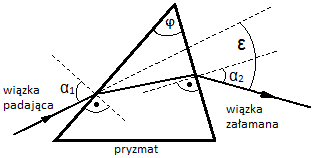
\includegraphics[width=0.5\textwidth]{./epsilon.png}
  \caption{Kąt odchylenia $\varepsilon$ wiązki światła przy przechodzeniu przez pryzmat.}
  \label{}
\end{figure}

Kąt odchylenia $\varepsilon$ zależy m.in. on od kąta padania $\alpha$ i jest najmniejszy w sytuacji, gdy kąt padania $\alpha_1$ i kąt wyjścia $\alpha_2$ są równe. Jest to tzw. "przebieg symetryczny", dla którego, w oparciu o prawo Snelliusa, zachodzi równość:
 \begin{equation}
n = \frac{\sin \frac{\varepsilon_{min}+\varphi}{2}}{\sin \frac{\varphi}{2}}
\end{equation}
\begin{figure} [H]
  \centering
  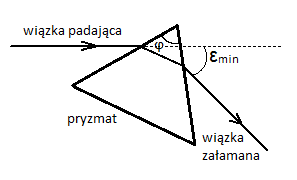
\includegraphics{./epsilon_min.png}
  \caption{Kąt najmniejszego odchylenia $\varepsilon_{min}$ dla tzw. przebiegu symetrycznego.}
  \label{}
\end{figure}

\section{Opis układu i metody pomiarowej}


\section{Wyniki pomiarów}
Kąt łamiący pryzmatu: $60^\circ$
Kąt zerowy: $45^\circ 30'$
\subsection{Pomiary dla sodu}
\begin{itemize}
  \item żółty (dlugość fali) $346^\circ 50'$ %Nie przepisałyśmy długości fali, trzeba dopytac o to Marty
  \item zielony (dlugość fali) $145^\circ 30'$
\end{itemize}
\subsection{Pomiary dla neonu}
\begin{tabular}{lrrr}
{} &  $\lambda[nm]$ &  $\alpha[^\circ]$ &  $\alpha[']$ \\
0  &         654 &          348 &          18 \\
1  &         651 &          348 &          10 \\
2  &         641 &          348 &           0 \\
3  &         614 &          347 &          46 \\
4  &         610 &          347 &          40 \\
5  &         603 &          347 &          26 \\
6  &         591 &          347 &          10 \\
7  &         588 &          347 &           0 \\
8  &         540 &          346 &          20 \\
9  &         534 &          346 &          10 \\
10 &         470 &          345 &          48 \\
11 &         454 &          344 &          44 \\
\end{tabular}

\section{Analiza pomiarów}
%Do wykresu dorobię jeszcze dopasowaną krzywą i zrzutuję nań pomiary z sodu i naniosę niepewności
\begin{figure} [H]
  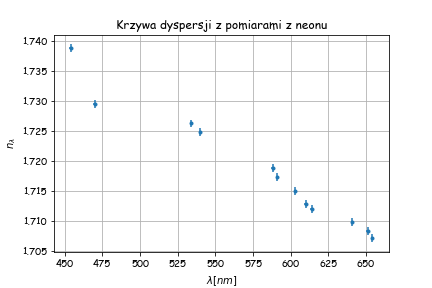
\includegraphics{./dyspersja.png}
  \caption{}
  \label{}
\end{figure}

\section{Analiza niepewności}
Za niepewność pomiaru wzięto:
\begin{equation}
  \Delta \alpha = \sqrt{(\frac{\Delta_k}{3})^2+(\frac{\Delta_o}{3})^2}
\end{equation}
gdzie $\Delta_k$ - podziałka kątomierza: $2'$, a $\Delta_o$ - niepewność eksperymentatora: $2'$.\\
Dalsze niepewności wyliczano metodą propagacji niepewności:
\begin{itemize}
  \item Kąt łamiący pryzmatu
  \begin{equation}
    \Delta \varphi = \sqrt{(\frac{\Delta \alpha_L}{2})^2+(\frac{\Delta \alpha_P}{2})^2}
  \end{equation}
  \item Kąt najmniejszego odchylenia
  \begin{equation}
    \Delta \varepsilon_{min} = \sqrt{(\Delta \alpha)^2+(\Delta \alpha_0)}
  \end{equation}
  \item Wspołczynnik załamania
  \begin{equation}
    \Delta n = \sqrt{(\Delta \varphi \frac{\sin{\left (\frac{\varepsilon_{min}}{2} \right )}}{\cos{\left (\phi \right )} - 1})^2+
    (\Delta \varepsilon \frac{\cos{\left (\frac{\varepsilon_{min}}{2} + \frac{\phi}{2} \right )}}{2 \sin{\left (\frac{\phi}{2} \right )}})^2}
  \end{equation}
\end{itemize}

\section{Wnioski}


\end{document}
